\section{Analisis Data dan Hasil Komputasi}

\subsection*{Rekam Jejak Konvergensi Iterasi Newton-Raphson Multivariat}
Loop optimasi Newton-Raphson multivariat dieksekusi dengan kriteria toleransi henti ganda $\varepsilon = 10^{-6}$. Solusi mencapai konvergensi penuh hanya dalam 6 langkah iterasi. Ringkasan dinamika komputasi numerik pada tiap langkah disajikan pada Tabel~\ref{tab:konvergensi_newton}.

\begin{table}[H]
    \centering
    \small
    \setlength{\tabcolsep}{4pt}
    \caption{Riwayat konvergensi numerik algoritma Newton-Raphson multivariat.}
    \label{tab:konvergensi_newton}
    \begin{tabular}{c S[table-format=2.4] S[table-format=1.4e2] S[table-format=1.4e2] S[table-format=1.2e2] S[table-format=1.6] S[table-format=1.6]}
        \toprule
        {Iterasi ($k$)} & {$\chi^2$ Total} & {$\|\mathbf{g}\|_2$} & {$\|\Delta\mathbf{p}\|_2$} & {$\kappa(\mathbf{H})$} & {$E_r$ (\si{\mega\electronvolt})} & {$\Gamma$ (\si{\mega\electronvolt})} \\
        \midrule
        0 & 90.8117 & 1.8612e+04 & 1.6565e-01 & 8.75e+03 & 2.070000 & 0.060000 \\
        1 & 19.6202 & 1.4073e+03 & 4.1345e-02 & 6.42e+03 & 2.072851 & 0.067405 \\
        2 & 18.6204 & 1.4903e+02 & 2.5940e-03 & 6.86e+03 & 2.073011 & 0.065678 \\
        3 & 18.6066 & 1.5155e+01 & 3.9396e-04 & 6.80e+03 & 2.073019 & 0.065920 \\
        4 & 18.6064 & 1.8316e+00 & 4.6755e-05 & 6.81e+03 & 2.073019 & 0.065891 \\
        5 & 18.6064 & 2.2327e-01 & 5.6582e-06 & 6.81e+03 & 2.073019 & 0.065895 \\
        6 & 18.6064 & 2.6967e-02 & 0.0000e+00 & 6.81e+03 & 2.073019 & 0.065895 \\
        \bottomrule
    \end{tabular}
\end{table}

Penurunan nilai $\chi^2$ dari $90.8117$ menjadi $18.6064$ berlangsung sangat cepat pada iterasi ke-1 dan ke-2. Norma langkah koreksi $\|\Delta\mathbf{p}\|_2$ menyusut secara kuadratik dari $1.65 \times 10^{-1}$ hingga di bawah batas toleransi $10^{-6}$, membuktikan tercapainya konvergensi kuadratik orde-dua yang menjadi karakteristik unggul dari metode Newton-Raphson berbasis matriks kelengkungan eksak.

\subsection*{Hasil Akhir Estimasi Parameter Fisis dan Derajat Kebebasan}
Berdasarkan $N = 59$ titik data dan $m = 4$ parameter yang diestimasi, derajat kebebasan sistem adalah:
\begin{equation}
    \nu = N - m = 59 - 4 = 55
\end{equation}
Nilai kelayakan \textit{reduced chi-square} optimal diperoleh sebesar:
\begin{equation}
    \chi^2_{red} = \frac{\chi^2_{\min}}{\nu} = \frac{18.6064}{55} \approx 0.3383
\end{equation}

Ringkasan nilai parameter fisis optimal hasil konvergensi beserta simpangan baku ketidakpastian statistik disajikan pada Tabel~\ref{tab:parameter_optimal}.

\begin{table}[H]
    \centering
    \small
    \setlength{\tabcolsep}{6pt}
    \caption{Hasil estimasi parameter fisis penampang lintang resonansi $^{12}\text{C}(n,\text{tot})$.}
    \label{tab:parameter_optimal}
    \begin{tabular}{l c c c}
        \toprule
        \textbf{Parameter Fisis} & \textbf{Simbol} & \textbf{Nilai Optimal $\pm$ Ketidakpastian} & \textbf{Galat Relatif} \\
        \midrule
        Energi Resonansi Pusat & $E_r$ & \SI{2.073019 \pm 0.000379}{\mega\electronvolt} & \SI{0.018}{\percent} \\
        Lebar Spektral Resonansi & $\Gamma$ & \SI{0.065895 \pm 0.001148}{\mega\electronvolt} & \SI{1.74}{\percent} \\
        Amplitudo Resonansi Puncak & $\sigma_0$ & \SI{3.133715 \pm 0.030648}{\barn} & \SI{0.98}{\percent} \\
        Kontinum Latar Belakang & $\sigma_{bg}$ & \SI{4.587609 \pm 0.008926}{\barn} & \SI{0.19}{\percent} \\
        \bottomrule
    \end{tabular}
\end{table}

\subsection*{Matriks Kovariansi dan Matriks Korelasi Ternormalisasi}
Matriks kelengkungan Hessian pada titik optimal $\mathbf{H}(\mathbf{p}^*)$ memiliki determinan positif dengan bilangan kondisi teratur $\kappa(\mathbf{H}) = 6.81 \times 10^3$. Inversi matriks menghasilkan matriks kovariansi parameter asimptotik $\mathbf{C} = 2[\mathbf{H}(\mathbf{p}^*)]^{-1}$:
\begin{equation}
    \mathbf{C} = \begin{pmatrix}
     4.249 \times 10^{-7} &  1.082 \times 10^{-7} & -6.311 \times 10^{-6} & -1.503 \times 10^{-7} \\
     1.082 \times 10^{-7} &  3.896 \times 10^{-6} & -4.910 \times 10^{-5} & -1.749 \times 10^{-5} \\
    -6.311 \times 10^{-6} & -4.910 \times 10^{-5} &  2.777 \times 10^{-3} & -7.868 \times 10^{-5} \\
    -1.503 \times 10^{-7} & -1.749 \times 10^{-5} & -7.868 \times 10^{-5} &  2.355 \times 10^{-4}
    \end{pmatrix}
    \label{eq:matrix_C_val}
\end{equation}

Normalisasi elemen kovariansi menghasilkan matriks korelasi parameter $\boldsymbol{\rho}$ sebagaimana disajikan pada Tabel~\ref{tab:matriks_korelasi}.

\begin{table}[H]
    \centering
    \small
    \setlength{\tabcolsep}{6pt}
    \caption{Matriks korelasi silang ternormalisasi antar-parameter ($\boldsymbol{\rho}$).}
    \label{tab:matriks_korelasi}
    \begin{tabular}{l S[table-format=-1.4] S[table-format=-1.4] S[table-format=-1.4] S[table-format=-1.4]}
        \toprule
        \textbf{Parameter} & {$E_r$} & {$\Gamma$} & {$\sigma_0$} & {$\sigma_{bg}$} \\
        \midrule
        $E_r$       &  1.0000 &  0.0842 & -0.1846 & -0.0150 \\
        $\Gamma$    &  0.0842 &  1.0000 & -0.4737 & -0.5754 \\
        $\sigma_0$  & -0.1846 & -0.4737 &  1.0000 & -0.0965 \\
        $\sigma_{bg}$ & -0.0150 & -0.5754 & -0.0965 &  1.0000 \\
        \bottomrule
    \end{tabular}
\end{table}

\subsection*{Visualisasi Hasil Fitting Resonansi dan Metrik Konvergensi}
Grafik hasil fitting penampang lintang Breit-Wigner beserta panel evaluasi distribusi residu terstandarisasi disajikan pada Gambar~\ref{fig:resonance_fit}.

\begin{figure}[H]
    \centering
    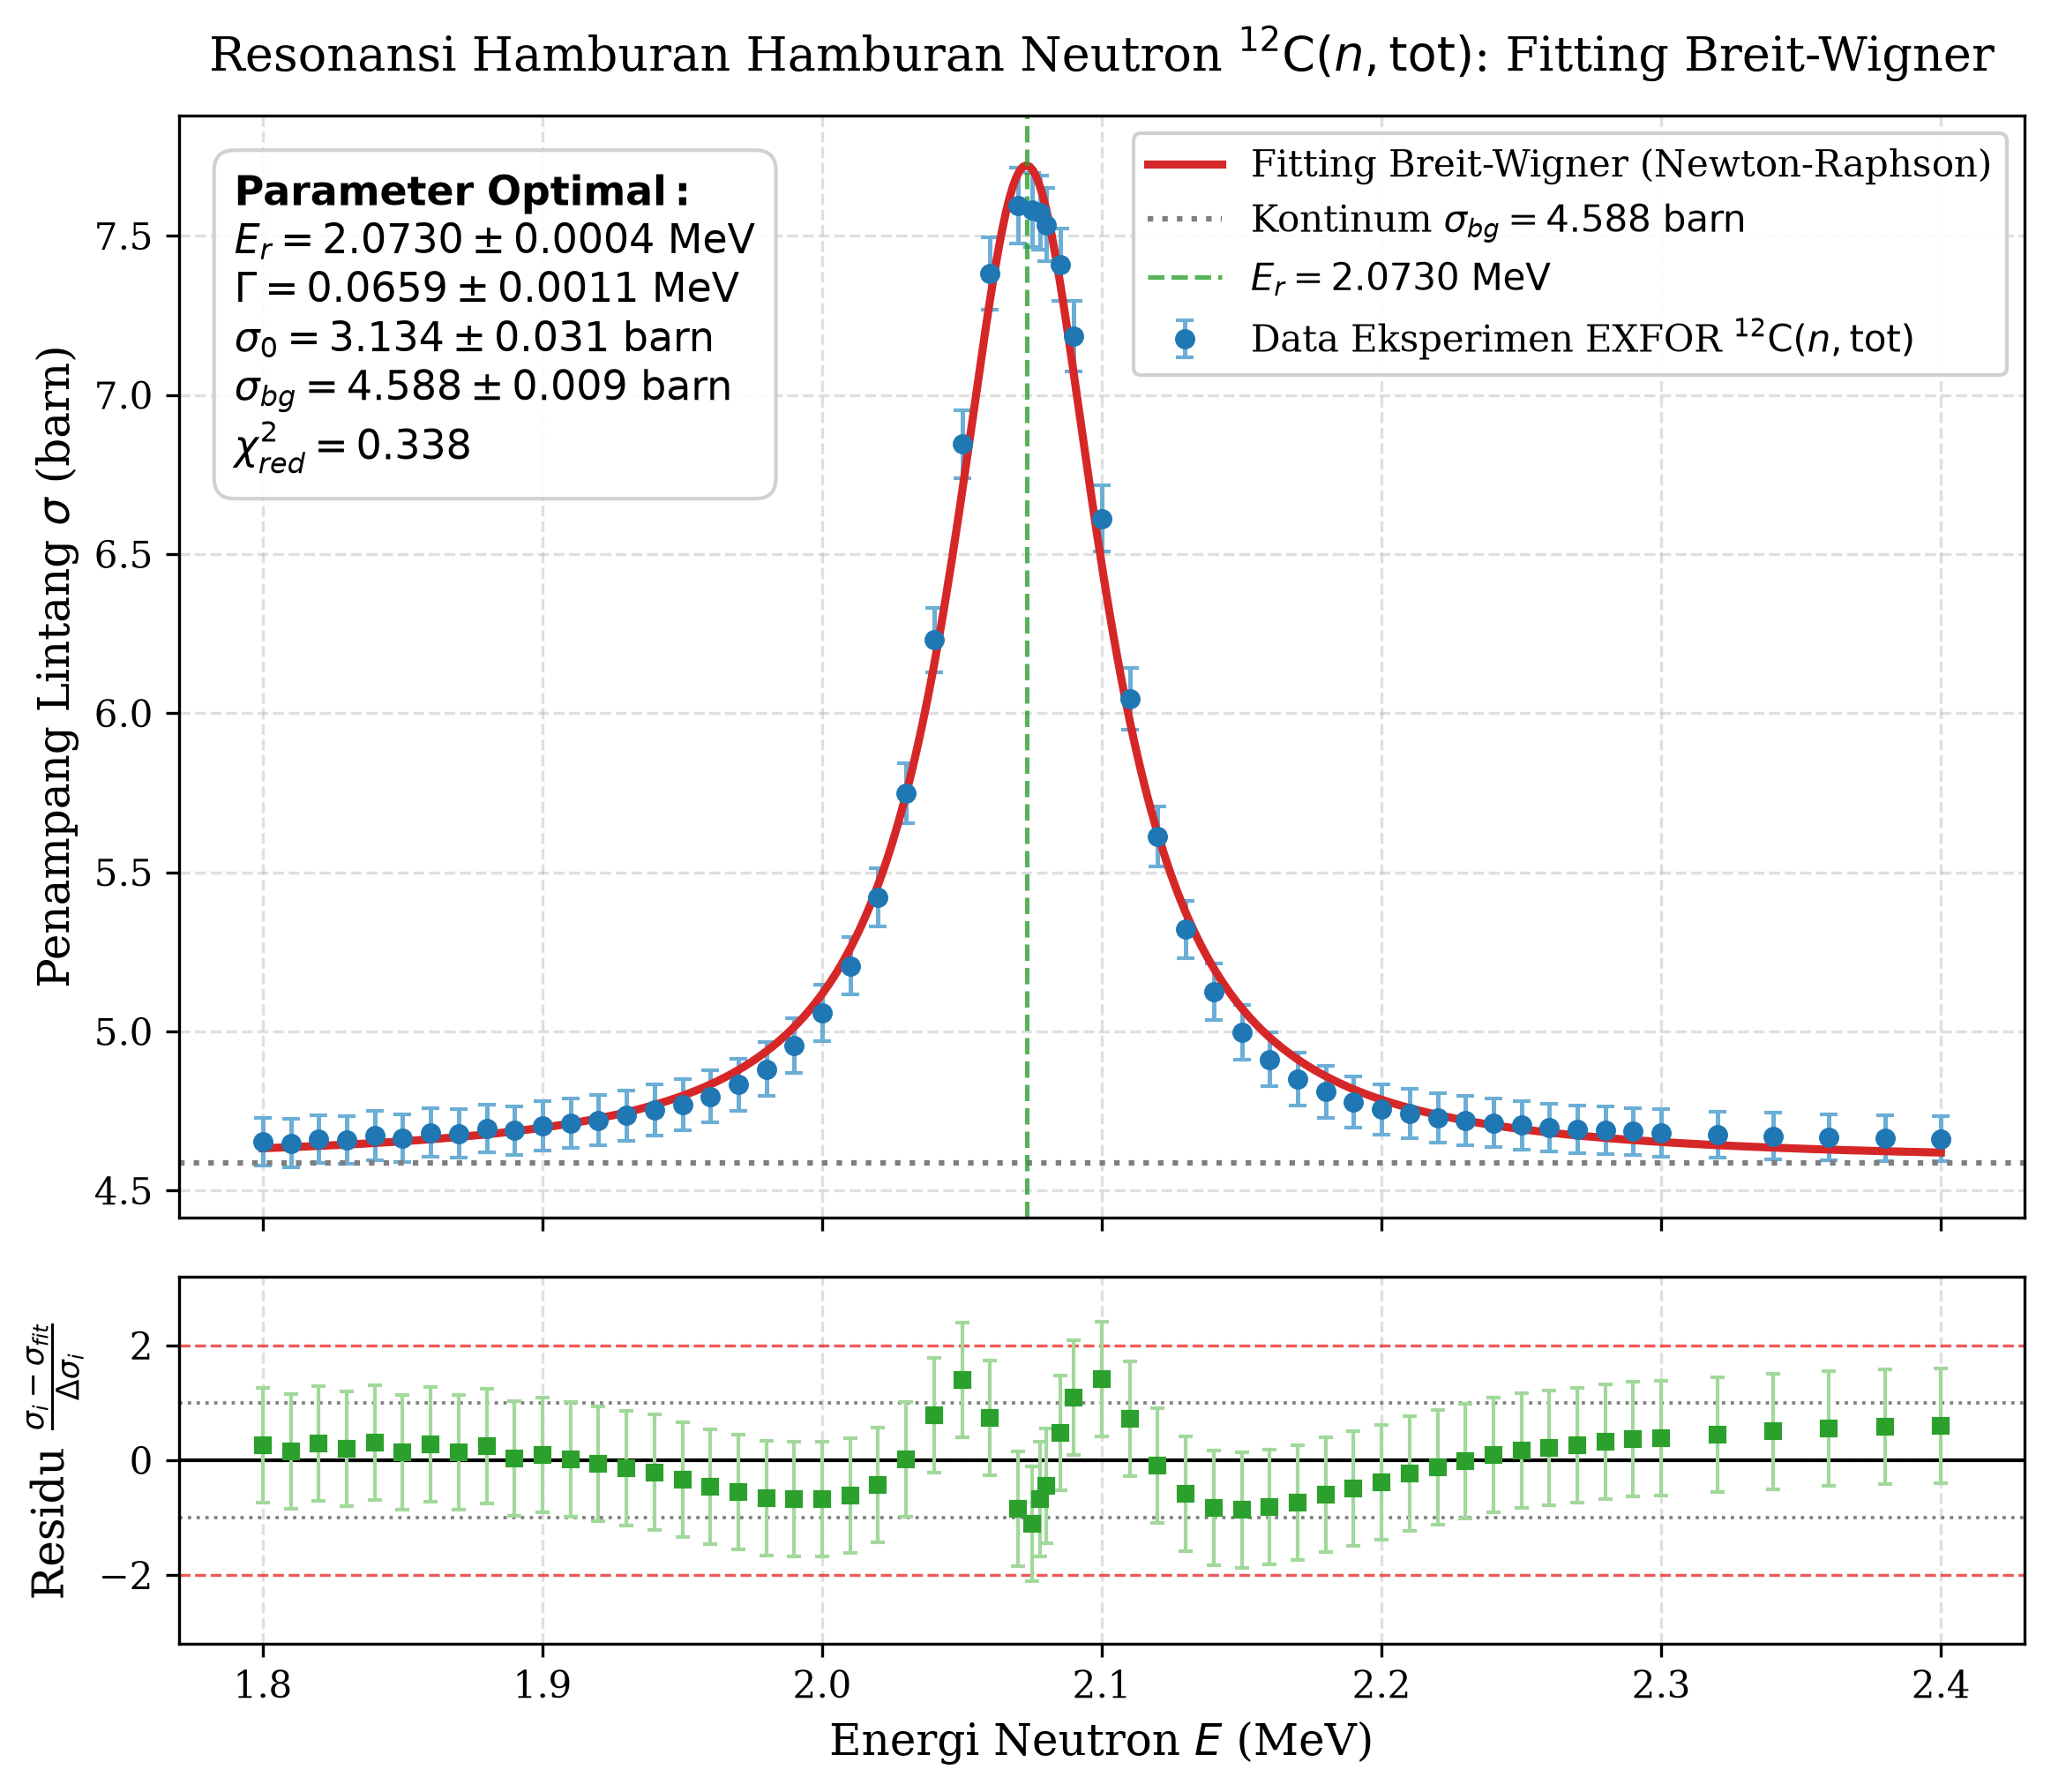
\includegraphics[width=0.88\textwidth]{resonance_fitting_plot.png}
    \caption{Grafik fitting kurva Breit-Wigner terhadap data eksperimen $^{12}\text{C}(n,\text{tot})$ (panel atas) dan distribusi residu terstandarisasi $R_i = (\sigma_i - \sigma_{fit})/\Delta\sigma_i$ (panel bawah).}
    \label{fig:resonance_fit}
\end{figure}

Dinamika laju konvergensi kuadratik semilogaritmik serta evolusi bilangan kondisi Hessian $\kappa(\mathbf{H})$ disajikan pada Gambar~\ref{fig:convergence_metrics}.

\begin{figure}[H]
    \centering
    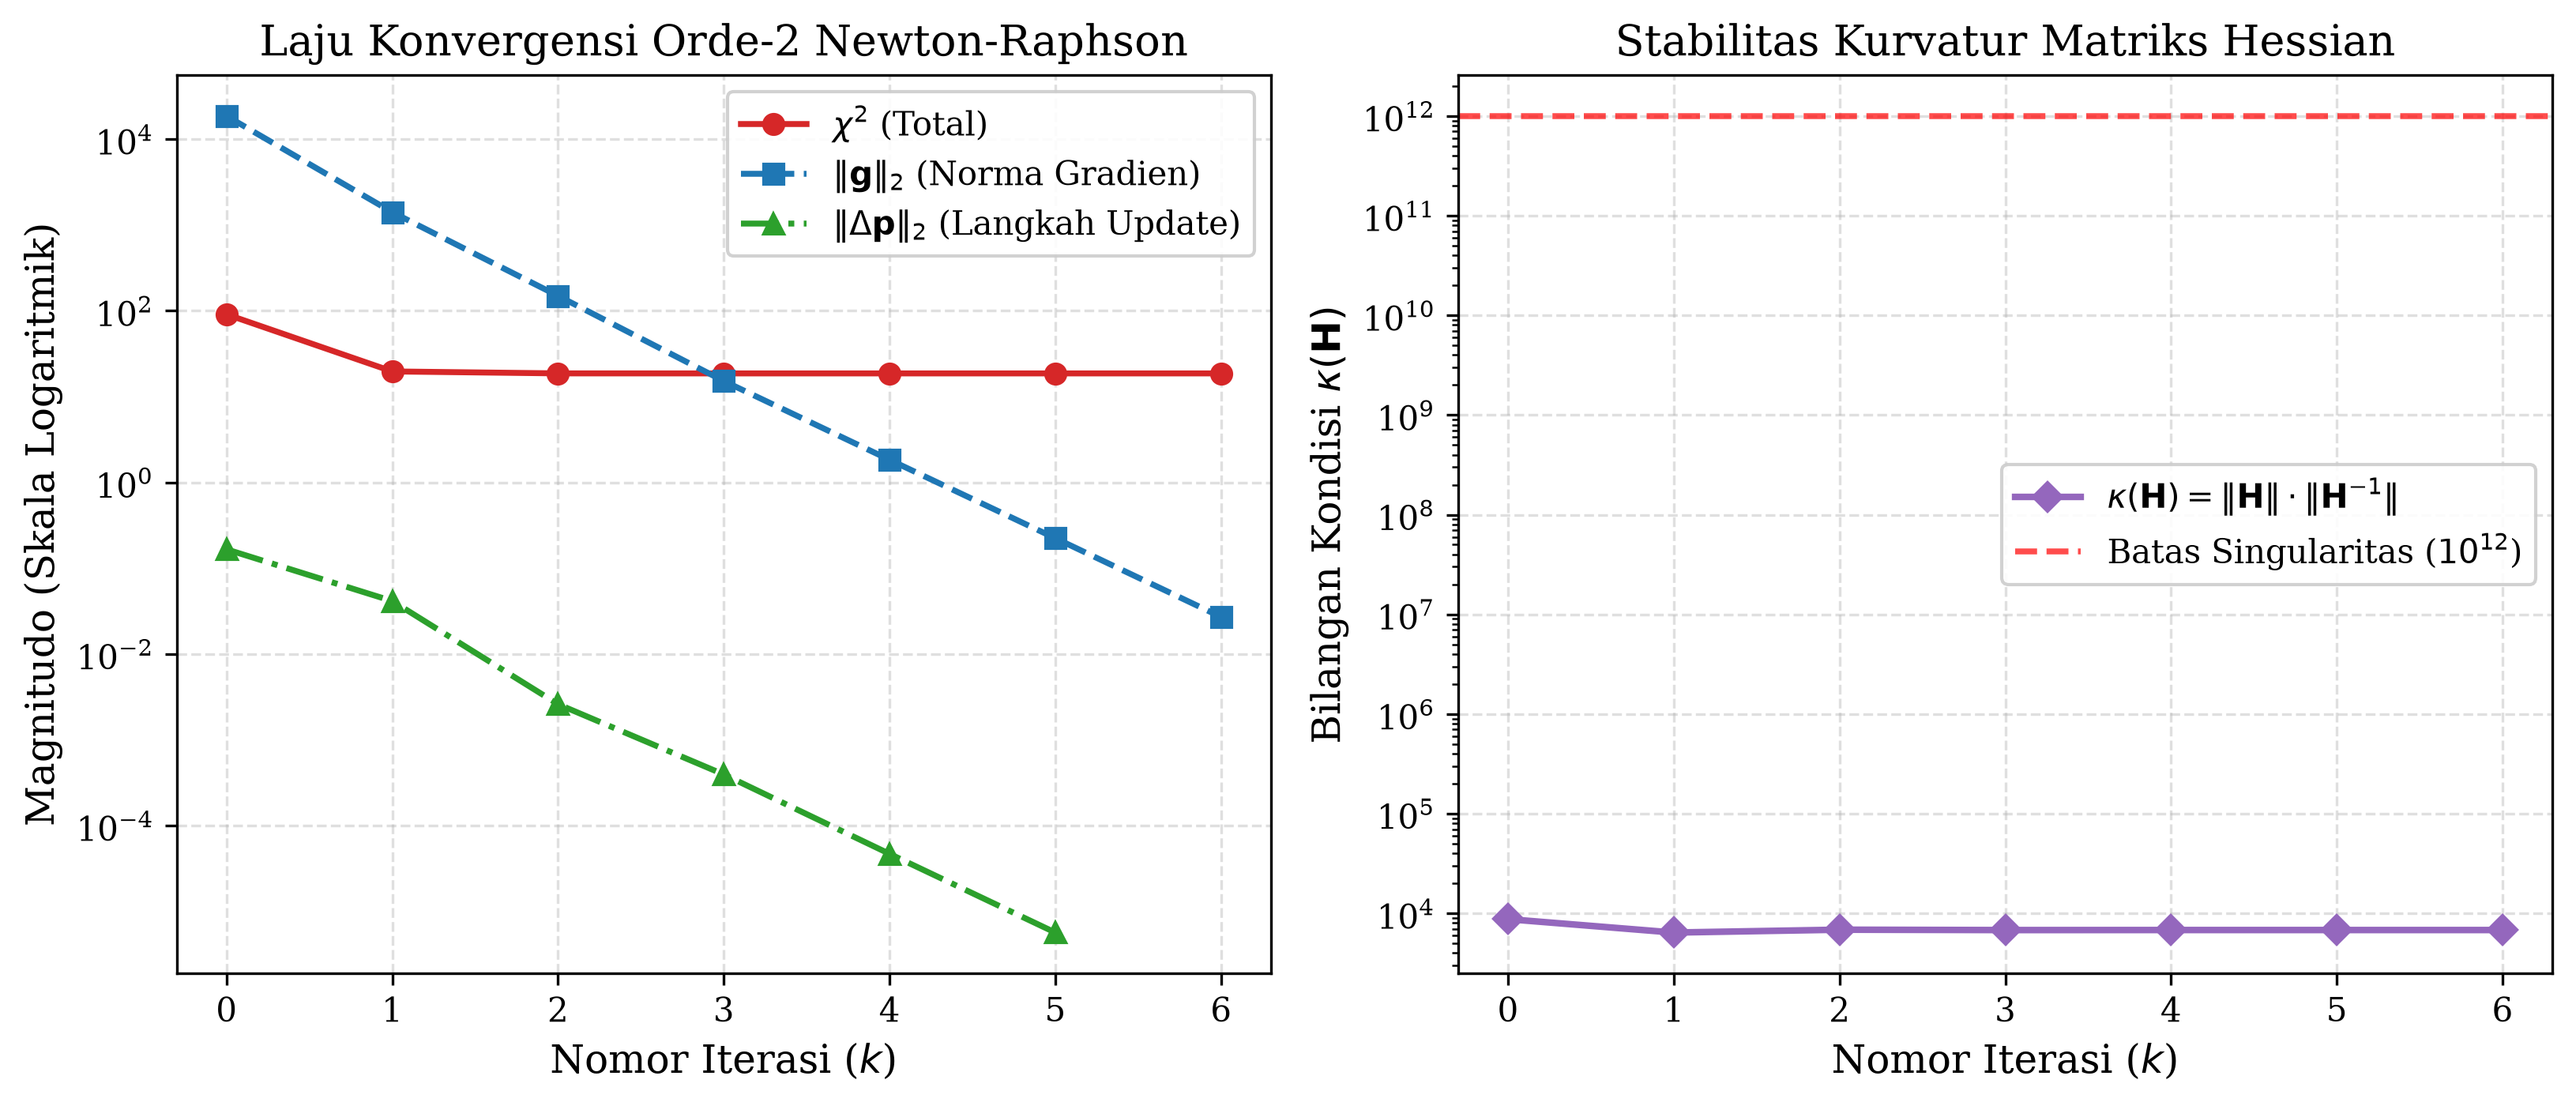
\includegraphics[width=0.95\textwidth]{convergence_metrics_plot.png}
    \caption{Profil laju konvergensi orde kedua Newton-Raphson: peluruhan kuadratik $\chi^2$, norma gradien, dan langkah update (panel kiri) serta dinamika kestabilan bilangan kondisi $\kappa(\mathbf{H})$ (panel kanan).}
    \label{fig:convergence_metrics}
\end{figure}
